\documentclass[a4paper]{article}

%% Language and font encodings
\usepackage[english]{babel}
\usepackage[utf8x]{inputenc}
\usepackage[T1]{fontenc}

%% Sets page size and margins
\usepackage[a4paper,top=3cm,bottom=2cm,left=3cm,right=3cm,marginparwidth=1.75cm]{geometry}

%% Useful packages
\usepackage{amsmath}
\usepackage{enumerate}
\setlength\parindent{0pt}
\usepackage{amssymb}
\usepackage{graphicx}
\usepackage{float}

\setcounter{section}{-1}
\title{MA 1971 Exercise Set 5 Answers}
\author{Hubert J. Farnsworth}

\begin{document}
\maketitle

\begin{enumerate}
%%%%%%%%%%%%%%%%%%%%%
%%%%%%%%  1  %%%%%%%%
%%%%%%%%%%%%%%%%%%%%%
\item

Show that the harmonic mean is less than or equal to the geometric mean. Hint:
Let bk := 1/ak and apply the relationship between the geometric mean and the
arithmetic mean to the bk.

Let $a_1, \dots , a_n > 0$ and define $b_k := 1/a_k$ for $k = 1, \dots , n$. We proved in lecture 19 that the geometric mean is less than or equal to the arithmetic mean: $\sqrt[n]{b_1b_2 \dots b_n} \leq (b_1 + b_2 \dots + b_n)/n$. 

\begin{align*}
\frac{n}{1/a_1 + 1/a_2 + \dots + 1/a_n} &=
\frac{n}{b_1 + b_2 + \dots + b_n} \\
&\leq \frac{1}{\sqrt[n]{b_1b_2 \dots b_n}} \\
& = (b_1b_2 \dots b_n)^{-\frac{1}{n}} \\ 
&= (a_1^{-1}a_2^{-1} \dots a_n^{-1})^{-\frac{1}{n}} \\
&=((a_1a_2 \dots a_n)^{-1})^{-\frac{1}{n}} \\
&= (a_1a_2 \dots a_n)^{\frac{1}{n}} \\
&= \sqrt[n]{a_1a_2\dots a_n} \;.
\end{align*}


\newpage
%%%%%%%%%%%%%%%%%%%%%
%%%%%%%%  2  %%%%%%%%
%%%%%%%%%%%%%%%%%%%%%
\item

Draw all of the possible graphs on four vertices. Which ones are connected and
which are disconnected?

	\begin{figure}[H]
	\centering
  	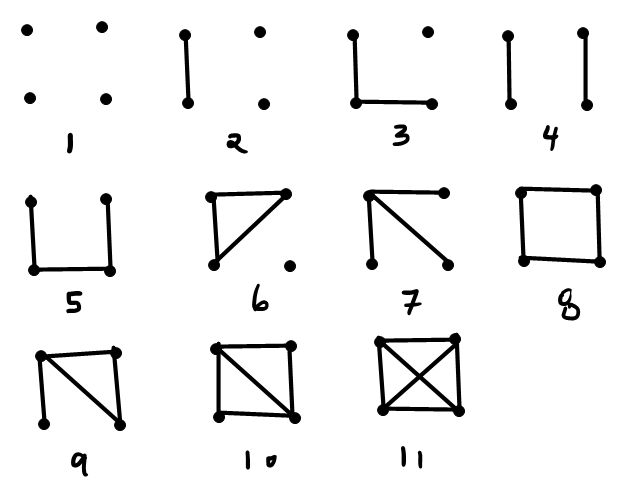
\includegraphics[width=0.65\linewidth]{HW5Exercise2.png}
	\end{figure}
	
	There are 11 possible graphs up to isomorphism.
	Graphs 5,7,8,9,10, and 11 are connected graphs.


\newpage
%%%%%%%%%%%%%%%%%%%%%
%%%%%%%%  3  %%%%%%%%
%%%%%%%%%%%%%%%%%%%%%
\item

A walk is a alternating sequence of vertices and incident edges of the form
$$
\{v_0, e_1, v_1, e_2, v_2, \dots , e_n, v_n \}
$$
where repetition is allowed. A closed walk is a walk which begins and ends at the same vertex

\begin{enumerate}
	\item
	Please give an example of a closed walk with an even number of edges
	which contains no cycle. \\
	
	Consider $\{v_0 , e_1, v_1, e_2, v_2, e_2, v_1, e_1, v_0\}$. This
	is a closed walk with four edges. It contains no cycles. We assume
	cycles must by definition have at least 3 edges so that $\{v_1, e_2,
	v_2, e_2, v_1 \}$, for example, is not a cycle. 
	
	\item
	Please show that any closed walk with an odd number of edges must
	contain an (odd) cycle. \\
	
	Given a graph $G$, suppose there is a closed walk with an odd number of edges. If all vertices are distinct (except for the first and last), then this walk is itself an odd cycle, and we are done. If not, then there is at least one vertex that repeats in the middle of the walk. Use this vertex to divide our original close walk into 2 or more closed subwalks. Notice that at least one of these subwalks is odd. Pick one of the shortest odd subwalks. If this chosen subwalk is a cycle, we are done. If not, continue the process. This process must terminate and must terminate with an odd cycle. Conclude that if a graph contains a closed walk with an odd number of edges, then this closed odd walk must contain an odd cycle. 
	
\end{enumerate}


\newpage
%%%%%%%%%%%%%%%%%%%%%
%%%%%%%%  4  %%%%%%%%
%%%%%%%%%%%%%%%%%%%%%
\item

Please show that any planar graph must have a vertex with degree that is less than or equal to 5. \\

We use a proof by contradiction. Recall the Euler formula $|V| - |E| + |F| = 2$. Because every edge is associated,

$$ \sum_{k=1}^n \text{deg}(v_k) = 2|E|, \quad n := |V| \;.$$

Suppose the minimum degree of any vertex in our graph is six. Then

$$ 6|V| \leq \sum_{k=1}^n \text{deg}(v_k) = 2|E| \implies |V| \leq \frac{1}{3}|E| \;.$$

Next note that each face is bounded by at least 3 edges while each edge is associated with 2 faces while each edge is associated with 2 faces. Thus $3|F| \leq 2|E|$ so that $|F| \leq \frac{2}{3}|E|$. Therefore,

$$
2 = |V| - |E| + |F| 
\leq \frac{1}{3}|E| - |E| + \frac{2}{3}|E| = 0 \;.
$$

The contradiction $2 = 0$ arose from the assumption that all vertices in our graph have degree at least 6. This assumption must be false, so we conclude that there must be a vertex with degree 5 or less. 



\end{enumerate}

\end{document}